% Set title page for separate titlepage
\documentclass[titlepage]{report}

%---------% Packages %---------%
% Some standard math packages
\usepackage{amsmath}
\usepackage{amssymb}
\usepackage{amsfonts}
\usepackage{amsthm}
\usepackage{IEEEtrantools}

% Package for lists
\usepackage[shortlabels]{enumitem}

% Graphics
\usepackage{graphicx}
\usepackage{subcaption}
\usepackage{tikz}
\usetikzlibrary{fit,
						backgrounds,
						arrows,
						decorations.markings,
						decorations.pathmorphing,
						snakes,
						shapes.misc, 
						positioning,
						scopes,
						calc}

\tikzset{colorbox/.style={thick, rounded corners=2pt, text height=1.7ex,text depth=.25ex, draw=#1!70!black, fill=#1!30}}

\tikzset{colorelement/.style={thick, rounded corners=2pt, draw=#1!70!black, fill=#1!30}}
\tikzset{conn/.style={thick, shorten <=#1, shorten >=#1}}
\tikzset{arr_node/.style={pos=0.5,above,font=\scriptsize, sloped}}

\usepackage{float}
\usepackage{multirow}
%\usepackage{gnuplot-lua-tikz}

% Utilities
\usepackage{lipsum}
\usepackage{arydshln}

% Biblatex
\usepackage[backend=biber,style=numeric,sorting=nty]{biblatex}
\nocite{*}
\addbibresource{bib/references.bib}

% Appendices
\usepackage[toc]{appendix}
%------------------------------------%

% Math environments
\theoremstyle{remark}
\newtheorem{remark}{Remark}
\newtheorem{xmpl}{Example}
\newtheorem{definition}{\textbf{Definition}}

%quantum commands
\renewcommand{\H}{\mathcal{H}}
\newcommand{\ket}[1]{|#1 \rangle}
\newcommand{\bra}[1]{\langle #1|}
\newcommand{\braket}[2]{\langle#1|#2\rangle}
\newcommand{\bk}[2]{\langle#1|#2\rangle}
\newcommand{\ketbra}[2]{|#1 \rangle\langle #2|}
\newcommand{\kb}[2]{|#1 \rangle\langle #2|}
\newcommand{\proj}[1]{|#1\rangle\langle #1|}

%Math commands
\DeclareMathOperator{\Tr}{Tr} % Trace
\DeclareMathOperator{\Ent}{H} % Entropy
\DeclareMathOperator{\I}{I} % Mutual Information
\newcommand{\keyrate}[3]{S(#1;#2||#3)} % secret key rate
\newcommand{\intrinfo}[3]{\I(#1;#2\!\downarrow\!#3)} % intrinsic information
\newcommand{\redintrinfo}[3]{\I(#1;#2\!\downdownarrows\!#3)} %reduced intrinsic information

%------------------------------------%

\begin{document}

\begin{titlepage}
    \begin{center}
        \vspace*{1cm}
        
        \Huge
        \textbf{Bound Information}
        
        \vspace{0.5cm}
        \LARGE
        {Analysis of a Classical Analogue to Bound Entanglement}
        
        \vspace{1.5cm}
        
        \textbf{Luca Dolfi}\\ 
         Advisor: Prof. Stefan Wolf \\ 
         Tutor: Arne Hansen \\
        
        \vfill
        
        A thesis presented for the degree of\\
        BSc in Informatics
        
        \vspace{0.8cm}
        
        \includegraphics[width=0.2\textwidth]{images/usi-immagini-logo-formatted.png}
        
        \Large
        Department of Informatics\\
        Universit\`a della Svizzera Italiana\\
        Spring 2018
        
    \end{center}
\end{titlepage}

\chapter*{Abstract}
%\begin{abstract}
There is a correspondence between entanglement distillation in quantum mechanics and classical key agreement in information theory. 
In the quantum-mechanical framework there are, furthermore, non-distillable, but entangled quantum states --- that is, states sharing bound entanglement. 
So, considering the above analogy, does there exists some notion of bound information? As of today this remains an open question.
In this project we follow the intuition from bound entanglement, the related measures and their connections to concepts of classical key agreement, as well as related information-theoretical concepts, in order to further investigate this open question.
We also look at a candidate probability distribution for bound information and perform numerical simulations in search for new, possibly better, candidates for bound information.\\

The structure of the report is as follows: 
after an explanation of the motivation of the search, chapter \ref{ch:two} explains the basics of key exchange in both classical and quantum mechanical frameworks.
 A comparison between methods is presented. 
 Chapters \ref{ch:three} and \ref{ch:four} give the foundations for information theoretical concepts needed to understand and work with theoretical security. 
 Chapter \ref{ch:five} summarizes the state of research on bound information and finally chapter \ref{ch:six} presents the numerical analysis conducted on probability distributions.
%\end{abstract}

%\chapter*{Acknowledgements}
%\lipsum[13]

\tableofcontents

%\chapter{Introduction}
%
\lipsum[3]
	\section{Basics of QM}
	\lipsum[7]
	\cite{QC10th}
		\subsection{Quantum Entanglement}
		\lipsum[4]
		\cite{4H07}
	\section{Basics of Information Theory}
	\lipsum[3]
		\subsection{Classical Key Agreement}
		\lipsum[3]

\chapter{Motivation}
% Motivation chapter
% contains also abstract explanation on theoretic secure key distribution

%\lipsum[3]

The goal of key exchange is to allow Alice and Bob to establish a secure, private channel for communication.
For two parties to communicate confidentially, it is first needed to share some secret key between them, so that each party can encrypt and decrypt the communication.
If two parties could not establish a secure initial key exchange, they cannot communicate securely without the risk of an eavesdropper Eve listening to them.
The ultimate goal of Alice and Bob is to achieve a level of privacy, such that no other Eve could have information about the communication, even partially.\\
The tools or \emph{resources} to obtain such initial common secret can have many shapes and forms in modern telecommunication, often relying on computer science.\\

It has been noticed that these concepts of privacy also appear in nature and the strongest analogy comes from quantum mechanics.\footnotemark 
From this theory arises the famous \emph{quantum entanglement} that appears to be the equivalent of privacy in many ways.
Both phenomena are composed of correlations between known parties that no other person can access or copy. As summed in \cite{4H07} "If systems are in pure entangled state then at the same time (i) systems are correlated and (ii) no other system is correlated with them.". 
This can be seen as Alice and Bob holding a secret that Eve can not get to know.
\begin{table}[h]
	 \centering
	 	\begin{tabular}{ l | l}
	 		\textbf{quantum theory} & \textbf{classical information} \\ 
	 		\hline 
	 		quantum entanglement & secret classical correlations \\ 
	 		quantum communication & secret classical communication \\ 
	 		classical communication & public classical communication \\ 
	 		entanglement distillation & classical key agreement (CKA) \\ 
	 		local actions & local actions \\ 
	 		bound entanglement & bound information ? \\
	 	\end{tabular} 
	 	\caption{Table showing key QM concepts and their analog in classical key agreement, following \cite{CP02}.
	 	\label{Tab:analogy}}
	 \end{table}
\\
\footnotetext{While those analogies are present in many sources, they can be found summed up in the paper by Collins and Popescu \cite{CP02}, which also shortly addresses the question of bound information. }

From table \ref{Tab:analogy} we see that some of the resources and operations of QM have a one-to-one analog in classical information theory. 
Such a close relation suggests that the two theories can be viewed together and to use one to better understand the other. 
It is important however to point out that quantum entanglement and its effects \emph{are not} a quantum manifestation of classical effects and one theory does not explain the other. \\
For example there is no known instance --- and it is believed to not exist -- of a classical correspondence to super-dense coding (a quantum effect). Other entities like a classical correspondence to bound entanglement, \emph{bound information}, are not excluded a priori and remain yet to be observed or disproved.\\

An open question has remained over the years asking whether bound information should exists in the classical regime.
Should this resource exists, it would be --- by definition --- unusable to generate any key from it.
While at first this might looks worthless, 
following the intuition from bound entanglement might lead to interesting bounds on information theoretical key exchange.\\

\paragraph*{The Question}
\begin{itemize}
		\item[] Is there a tripartite probability $P_{ABE}$, corresponding to Alice and Bob wanting to establish a key unknown to Eve, that has some \emph{cost} associated to it to create it, but has $0$ possible key bits extractable from it? 
\end{itemize}


	
		
% done
 \chapter{A Common Key Exchange Problem}
 %Foundations chapter
% contains fundamental and basic theories to approach the content later
%		(LinAlg)Notation (math framework for QM)
%		QM
%			Introduce first abstract QM on Hilbert space and then dirac
%		Information theory


\section{Mathematical Framework (for QM)}
	%TODO Correct and reformulate
	
		In order to understand subsequent sections of this thesis a basic knowledge of the mathematical framework behind quantum mechanics is needed.
		 It is also important to specify a standard notation as used in literature.
	
%	\begin{enumerate}
%	\item Dirac's braket notation
%	\item Inner/(Outer) product
%	\item Linear operator
%	\item Adjoints and Hermitian operators
%	\item Pauli matrices
%	\item Tensor Product and tensor space
%	\end{enumerate}
	
	\subsubsection*{Dirac's bra-ket notation and Hilbert spaces}
%	\begin{figure}[h!]
%		\centering
%		\includegraphics[scale=0.2]{images/sketch1.png} 
%		\caption{how a physical state is represented}
%	\end{figure}
	Every pure quantum state can be represented a vector in a vector space with inner product, i.e. a \emph{Hilbert space}. 
	The implication of this will be explained in the next section; for now we only look of this vector representation.\\
	 A complex Hilbert space $\H$ of dimension $n$ is isomorphic to $ \mathbb{C}^n $ with the standard inner product. 
	 In $\mathbb{C}^n $ one can choose a basis and represents vectors with coordinates with respect to this basis.\\
	The bra-ket notation is a handy notation introduced by physicist Paul Dirac to deal with such vector representation of quantum states. 
	First of all we note that a state $\varphi '\in\H$ corresponds via the isomorphism to $ \varphi  \in \mathbb{C}^n $. It can be represented as a vector with respect of some basis as follows
	$$\ket{\varphi} = \begin{pmatrix} \varphi_1 \\ \varphi_2 \\ \vdots \end{pmatrix}	  \text{  is a coloumn "ket" vector over } \H $$
	$$\bra{\varphi}  = \begin{pmatrix} \varphi_1 & \varphi_2 & \hdots \end{pmatrix} \text{  is a row "bra" vector over } \H $$
	To be representative of a quantum state the vector has to have unitary length, $\|\varphi\|= 1$.
	Furthermore the conjugate transpose of a \emph{bra} vector is the corresponding \emph{ket} vector, and vice versa.
	$$ \bra{\varphi}^{\dagger} = \ket{\varphi} \text{,    } \ket{\varphi}^{\dagger} = \bra{\varphi}$$
	More specifically, for a complex vector space as $\H$, the components of $\bra{\varphi}$ are each the complex conjugate of the components of $\ket{\varphi}$.\\
	It is worth noting that in quantum information we will consider only vectors of finite dimensions, and more often than not, the standard basis for qubits represented by
	$$\ket0 =  \begin{pmatrix} 1 \\ 0 \end{pmatrix}
	\text{ and }
	\ket1 =  \begin{pmatrix} 0 \\ 1 \end{pmatrix}$$
	which are recognizable as the equivalent of $\vec{e_1}$ and $\vec{e_2}$ in $\mathbb{C}^2$.\\
	
	To summarize then, $\ket{\varphi}$ represents a coloumn vector on a complex vector space with inner product equivalent to $\mathbb{C}^n$ in some basis, and $\bra{varphi}$ is its complex conjugate.
	
	
	\subsubsection*{Inner/outer product}
	%This one first to start from standard notation
	In standard vector notation we define the inner (scalar) product of complex vectors as
	$$ ( \vec{v}, \vec{w} ) =  \begin{pmatrix} \bar{v_1} & \bar{v_2}\end{pmatrix} \begin{pmatrix} w_1 \\ w_2 \end{pmatrix} = \begin{pmatrix} \bar{w_1} & \bar{w_2}\end{pmatrix} \begin{pmatrix} v_1 \\ v_2 \end{pmatrix} = ( \vec{w}, \vec{v} )^{\dagger}$$
	Written in bra-ket notation, the inner product of two state vectors $\ket{v}$ and $\ket{w}$ is
	$$ ( \ket{v} , \ket{w} ) = \bk{v}{w} = (\ket{w} , \ket{v} )^{\dagger} = \bk{w}{v}^{\dagger} $$
	Where $\dagger$ represents the conjugate transpose,	which produces a scalar (complex) value.\\ %real??
%	This property is fundamental in the sense that it will allows us to go from a state space --- that can be many dimensional --- to a \textit{measurement} space, which assumes real values.\\ %0 and 1 in our case??
	
	It is important also to note that through the inner product of two vectors we also define the norm $\|\ket{v}\|  =  \sqrt{\braket{v}{v}} $.\\
	
	
	The outer product of two vectors, on the other hand, produces a matrix, with very important properties. So if we define the matrix\footnote{The fact that the result of  $ \ketbra{w}{v} $ is indeed a matrix can be seen more directly if we remember that this is nothing less than a column-row vectors multiplication.} $A =  \ketbra{w}{v} $ we observe that
	$$ \ket{w}\braket{v}{v'} = \braket{v}{v'}\ket{w} $$	
	which is a convenient way of visualizing the action of matrix $A$. In particular if we divide it like $(\ketbra{w}{v}) (\ket{v'}) $ it is easy to interpret it as \textit{matrix $A$ acting on vector $\ket{v'}$}; but the other equivalent form $(\braket{v}{v'})(\ket{w})$ can also be seen as multiplying vector $\ket{w}$ by a value $\braket{v}{v'}$. \\
	%this part may be too similar to book, page 67...
	The meaning of this is that $\ketbra{w}{v}$ can indeed be defined as a (linear) operator from the vector space of $\ket{v}$ and $\ket{v'}$ to the vector space of $\ket{w}$. This comes in very handy when we later use it to define operations and measurements on quantum states.\\ % is this true?
	
	\subsubsection*{Linear operators}
	A linear operator between two vector spaces is defined as 
	$$ \mathbf{A}: V\longrightarrow W \text{  ,  }\ket{v_i}\mapsto A\ket{v_i}$$
	$$ \text{ linear in all inputs, i.e.  }  A\left( \sum_i a_i\ket{v_i}\right) = \sum_i a_i A\ket{v_i} \text{  for all } i $$ 
	Looking back at the definition of the matrix $ A = \ketbra{w}{v}$ we can now refer to it as a linear operator from now on. \\
	Some well-known linear operators acting on single qubits that we will use later on are the \textit{Pailu Matrices}
	$$ I = \begin{bmatrix} 1 & 0 \\ 0 & 1 \end{bmatrix}	 \quad   X = \begin{bmatrix} 0 & 1 \\ 1 & 0 \end{bmatrix}$$
	$$ Y= \begin{bmatrix} 0 & -i \\ i & 0 \end{bmatrix}	 \quad   Z = \begin{bmatrix} 1 & 0 \\ 0 & -1 \end{bmatrix}$$
	
	In particular it is safe to say that, unless stated otherwise, the operators that will be presented all have a set of properties and are called Hermitian operators, or self-adjoint operators.\\
	$$ A = A^{\dagger} \quad \Longrightarrow (A\ket{v})^{\dagger} = \bra{v}A^{\dagger} $$ 
	Operators have also to be positive, this means that it holds, for every $\ket{v}$ : $\bra{v}A\ket{v}$ is real non-negative. Any positive operator is also self-adjoint and therefore it has diagonal (spectral) representation $\sum_i \lambda_i \proj{i}$ with non-negative eigenvalues $\lambda_i$.\\
	
	\subsubsection*{Tensor product}
	The tensor product $V\otimes W$ is an operation between vector spaces that combines every element of the first vector space and every element of the second vector space in a bigger vector space. Tensor product is linear and from its properties emerges the famous phenomenon of quantum entanglement, which simply is that not all vectors in $\H = V\otimes W$ can be divided into $\ket{v}\otimes\ket{w}$ with $\ket{v}\in V,\; \ket{w}\in W$. This will later be explained in the next section.\\
	Notation and abbreviation for the tensor product is 
	$$ \ket{v}\otimes\ket{w} = \ket{v}\ket{w} = \ket{v,w} = \ket{vw}$$
	It has the following properties:
	\begin{description}
		\item $\forall\ket{v}\in V ,\; \forall\ket{w}\in W, \; \forall z\in \mathbb{C}$	\\
					$ z(\ket{v}\otimes\ket{w}) = (z\ket{v})\otimes\ket{w} = \ket{v}\otimes(z\ket{w} $
		\item $\forall\ket{v_1},\ket{v_2}\in V ,\; \forall\ket{w}\in W$	\\
					$ (\ket{v_1} + \ket{v_2})\otimes\ket{w} = \ket{v_1w} + \ket{v_2w} $
		\item $\forall\ket{v}\in V ,\; \forall\ket{w}\in W, \; A:V\rightarrow V' \; B:W\rightarrow W'$	\\
					$ (A\otimes B) \left(\sum_i a_i \ket{v_i w_i} \right) = \sum_i a_i A\ket{v_i}\otimes B\ket{w_i} $
	\end{description}
	The inner product on $V$ and $W$ can be used to define (linearly) an inner product on $V\otimes W$.	
	
\section{Quantum Mechanics}
	%TODO Correct and reformulate this
	
	\begin{quotation}
		The simplest quantum mechanical system, and the system which we will be most concerned with, is the \emph{qubit}. A qubit has a two-dimensional state space. [...] 
		The way a qubit differs from a bit is that superpositions of these two states, of the form $a\ket{0} + b\ket{1}$, can also exist, in which it is not possible to say that the qubit is definitely in the state $\ket0$, or definitely in the state $\ket1$.
		\cite{NC10}
	\end{quotation}
	
	\subsubsection*{The three postulates}
	\begin{quote}
		\textbf{Postulate 1}: Associated to any isolated physical system is a complex vector space with inner product (that is, a Hilbert space) known as the \emph{state space} of the system. 
		The system is completely described by its \emph{state vector}, which is a unit vector in the system's state space. \cite{NC10}
	\end{quote}
	
	\begin{quote}
		\textbf{Postulate 2}: The evolution of a \emph{closed} quantum system is described by a \emph{unitary transformation}. That is, the state $\ket{\psi}$ of the system at time $t_1$ is related to the state $\ket{\psi'}$ of the system at time $t_2$ by a unitary operator $U$ which depends only on times $t_1$ and $t_2$,
		$$ \ket{\psi'} = U\ket{\psi} $$
		\cite{NC10}
	\end{quote}
	
	\begin{quote}
		\textbf{Postulate 3}: Quantum measurements are described by a collection $\{M_m\}$ of \emph{measurements operators}. 
		These are operators acting on the state space of the system being measured. 
		The index $m$ refers to the measurement outcomes that may occur in the experiment. If the state of the quantum system is $\ket{\psi}$ immediately before the measurement then the probability that result $m$ occur is given by 
		$$ p(m) = \bra{\psi}M_m^{\dagger}M_m\ket{\psi} \: ,$$
		and the state of the system after the measurement is 
		$$ \frac{M_m\ket{\psi}}{\sqrt{\bra{\psi}M_m^{\dagger}M_m\ket{\psi}}} \: . $$
		The measurement operators satisfy the \emph{completeness equation},
		$$\sum_m  M_m^{\dagger}M_m = I \: .$$
		The completeness equation expresses the fact that probabilities sum to one:
		$$ 1 = \sum_m p(m) = \sum_m  \bra{\psi}M_m^{\dagger}M_m\ket{\psi} \: .$$ 
		\cite{NC10}
	\end{quote}
	
	Quantum mechanics is a very large and complex theory. For our purposes it is enough for us to only consider the quantum system called \emph{qubit} and its rules of computation following from the tensor product algebra.  ...
	
	%TODO review this
	All pure states in QM are normalized vectors in $\H$.
	$$ \ket{\psi} \text{ is a state vector } \Rightarrow \ket{\psi}\in\H \text{ and }  \vert\bk{\psi}{\psi}\vert = 1$$
	This is instrumental in seeing them as probability vectors. Every linear operator has then to be unitary to maintain this property.\\
	A statistical mixture of states corresponds to a \emph{density matrix}, which is itself a new state. It is important to note that a mixture of probability of states is not the same thing as superposition of states. In the latter we don't have a measure of uncertainty of the state, meaning also that in theory we are always able to find a measurement basis that will always output the same result for that state. In the former, however, this is not possible given by the direct intrinsic uncertainty of the state.\\
	Density matrices have then the properties:
	$$ M = \rho = \sum_i p_i \ketbra{\psi_i}{\psi_i} = \sum_i p_i P_{\ket{\psi_i}} \text{  , where state }\ket{\psi_i}\text{ has probability } p_i $$ 
	$\rho$ is a positive, trace-1 operator meaning that $\Tr{\rho} = 1$ and all eigenvalues of $\rho$ are positive. Moreover $\rho$ is a linear combination of projectors $\proj{\psi_i}$ which makes $\rho\in\mathbf{P}(\H)$ a projector itself on the the Hilbert space.
	
		\subsection{Quantum Measurements}
		To get an actual value out of a qubit one has to \textit{measure} it. Measurement is, mathematically, a projection onto some chosen computational basis. The result for each base vector projection is then interpreted as a \emph{probability}. The state then changes after measurement, meaning for example that it will not retain it value as superposition any more.\\
		...\\
		
		If Alice has the state $\ket{psi_i}$ out of $i=1..n$ and all states are orthonormal, then Bob can find out what the choice of $i$ was.
		If the states are not orthonormal there is no quantum measurement capable of distinguishing the states. \\
		From this follows that if the states $\ket{\psi_1}$ and $\ket{\psi_2}$ are not orthogonal, then $\ket{\psi_2}$ has a component orthogonal to $\ket{\psi_1}$ but also a component parallel to it which will give probability not $0$ of measuring differently.
		
			\quad\underline{Example:}\\
			\begin{center}
				$ Z = \begin{bmatrix} 1 & 0 \\ 0 & -1 \end{bmatrix} \quad P_{+1} = \proj{0} , \; P_{-1} = \proj{1}	 $\\
				Measurement on qubit $ \ket{\psi} = \frac{\ket0 + \ket1}{\sqrt{2}} $ has probability $p_{+1} = \bra{\psi}P_{+1}\ket{\psi} = \bk{\psi}{0}\bk{0}{\psi} = \frac{1}{2}$ and similarly $p_{-1} = \frac{1}{2}$
				\cite{NC10}
			\end{center}%!!taken from book!!

		\subsection{Quantum Entanglement}
		\begin{quotation}
		There exist vectors in $V\otimes W$ that can not be represented by a single tensor product:
		$$ \textrm{Given } v_1,v_2\in V \; w_1,w_2\in W \; \textrm{linear independent:}$$
		$$v_1\otimes w_1 + v_2\otimes w_2 = v_1w_1 + v_2w_2 \in V\otimes W \; \textrm{is \emph{not} separable}$$ 
		this may be strange because on physical level tensor product is combination(merging) of quantum systems
		\cite{Han13}
		\end{quotation}
		
		\begin{figure}[h]
			\centering
			%% Little schematics showing the origin of entanglement
%% from the linear theory of QM and tensor product

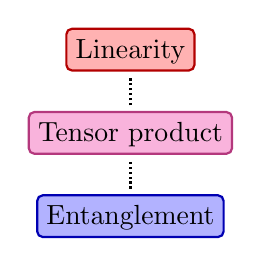
\begin{tikzpicture}[scale=0.6]
  \node[colorbox=red]                      (lin)  {Linearity};
  \node[colorbox=magenta, below=.5cm of lin] (tp)  {Tensor product};
  \node[colorbox=blue, below=.5cm of tp]   (en)  {Entanglement};
  \draw[conn=2pt, densely dotted] (tp) to (lin);
  \draw[conn=2pt, densely dotted] (en) to (tp);
\end{tikzpicture}
			\caption{origin of entanglement via linearity}
		\end{figure}
	
\section{Information Theory}
	
	\subsection{Mutual Information}
	Mutual information can be used as a measure of correlation between random variables. 
	
	Mutual information is defined as
	$$ I(X;Y) = \sum_{y\in\mathcal{Y}}\sum_{x\in\mathcal{X}} p(x,y) \log\left(\frac{p(x,y)}{p(x)p(y)}\right) $$
	or equivalently, showing its relation to the entropies of the random variables
	$$ I(X;Y) = H(X) - H(X\mid Y) = H(X,Y) - H(X\mid Y) - H(Y\mid X) $$
	This relation can be seen more directly in Fig. \ref{fig:mutual_info}.\\
	Mutual information is nonnegative and bounded by the entropy of random variable $X$
	$$ 0 \leq I(X;Y) \leq H(X) $$
	In this sense mutual information can also be interpreted as how much measuring one variable reduces the uncertainty of the other, thus being bounded by its uncertainty itself.
	
	\begin{figure}[h]
		\centering
		% Representation of mutual information in relation to entropy of variables
\tikzset{colorcircle/.style={circle, thick, minimum size=4cm, text height=1.7ex,text depth=.25ex, text width=3cm, draw=#1!70!black, fill=#1!30, fill opacity=0.33, text opacity=1.0}}

\begin{tikzpicture}[scale=0.6]
  \node[colorcircle=magenta] (Hx) at (-2,0)  {$ \Ent(X|Y) $ \hfill};
  \node[colorcircle=blue] (Hy) at (2,0)  {\hfill $ \Ent(Y|X) $};
  \node (mI) at (0,0) {$ \mathbf{\I(X;Y)} $};
  \node [left =of Hx.north] (HxL) {$ \Ent(X) $};
  \node [right =of Hy.north] (HyL) {$ \Ent(Y) $};
  \node (Hxy) at (0,-5.5) {$ \Ent(X,Y) $};
  \draw[->] (Hxy.north) -- ( Hx.south);
  \draw[->] (Hxy.north) -- (Hy.south);
  
  
%  \begin{scope}[shift={(8,2)}]
%    \draw[thick, draw=black, fill=white] (60:.75cm) arc (60:300:.75cm) (300:.75cm) arc (240:480:.75cm);
%    \node (Hxy) at (3,0) {$ \Ent(X,Y) $};
%  \end{scope}
  
\end{tikzpicture}

		\caption{Representation of mutual information $I(X;Y)$ in relation with entropies $H(X)$ and $H(Y)$ and joint entropy $H(X,Y)$ of the random variables .
		\label{fig:mutual_info}}
	\end{figure}		
	
	\subsection{Common Secret} \label{commonsecret}%here?
	Let $X,Y,Z,S$ be random variables on the same range $\mathcal{X}$. Let $X$ be owned by Alice, $Y$ by Bob and $Z$ by Eve. Then
	$$ (common) \qquad P[X=Y=S] > 1 - \epsilon $$
	$$ (secret) \qquad I(X;Z) = 0 \: \wedge \: I(Y;Z) = 0 $$
for all $\epsilon > 0 $. \\
The first part defines the \textit{common} property: $X$ and $Y$ must be asymptotically the same. 
The second part states that the amount of information Eve can gather about $X$ and $Y$, through it's realization of $Z$, is $0$.
% done
\chapter{Information Theoretical Model of Cryptography: Random Variables}
\section{Conjectures}
% Here you can retake the examples of protocols in chapter 1. After explaining Maurer postulate, show that they don't violate Maurer because of reasons.
			\begin{quotation}
			Bound entanglement is a kind of correlation between Alice and Bob inaccessible to Eve but nevertheless of no use for generating a secret (quantum) key.\\
			Unfortunately the existence of such bound information, which would contradict the mentioned conjecture\footnotemark on the classical side of the picture, could not be proven so far.
		\end{quotation}
		
		\footnotetext{Shannon: Information theoretical security can be achieved only by parties sharing an unconditionally secret key initially. Maurer: this key can also not be generated from scratch. Maurer+Wolf: \emph{Intrinsic information} between $A$ and $B$ given $E$ == \emph{secret key rate}(how much key can Alice and Bob generate from that $P_{ABE}$).}
		
	%\lipsum[1]
	\section{State of research}
		\begin{figure}[h]
			\centering
			% scheme representing the bounds
% expresed in paper Renner+Wolf 2003
% on the quantities intrinsic information,
% secret key rate and information of formaion

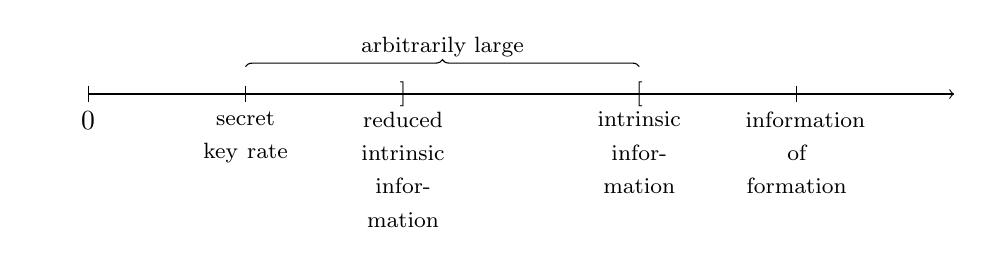
\begin{tikzpicture}

\tikzset{
    position label/.style={
       below = 3pt,
       align=center,
%       text height = 1.5ex,
%       text depth = 1ex,
       text width=13mm
    },
   brace/.style={
     decoration={brace},
     decoration={raise=3ex},
     decorate
   },
   blabel/.style={
		above = 13pt,
		align=center,
		pos=0.5   
   }
}

% draw horizontal line
\draw[->] (0,0) -- (11,0);

%draw vertical lines
\foreach \x in {0,2,9}
   \draw (\x cm,3pt) -- (\x cm,-3pt);
   
\node (foo) at (4cm,0) {\scalebox{0.9}{]}};
\node (bar) at (7cm,0) {\scalebox{0.9}{[}};

%labels
\node [position label] (Start) at (0,0) {$0$};
\node [position label] (skr) at (2,0) {\footnotesize secret key rate};
\node [position label] (rinf) at (4,0) {\footnotesize reduced intrinsic information};
\node [position label] (inf) at (7,0) {\footnotesize intrinsic information};
\node [position label] (iof) at (9,0) {\footnotesize information of formation};

\draw [brace] (skr.north) -- node [blabel] {\footnotesize arbitrarily large} (inf.north);

\end{tikzpicture}
			\caption{Bounds on the quantities as stated in Wolf + Renner 2003 proceeding}
		\end{figure}
	%\lipsum[1]
	\section{My considerations}
	%\lipsum[1]

% done
\chapter{Measures of Correlation and Their Bounds}
\section{Mutual Information}
    Mutual information can be used as a measure of correlation between random variables. 
	
	Mutual information is defined as
	$$ I(X;Y) = \sum_{y\in\mathcal{Y}}\sum_{x\in\mathcal{X}} p(x,y) \log\left(\frac{p(x,y)}{p(x)p(y)}\right) $$
	or equivalently, showing its relation to the entropies of the random variables
	$$ I(X;Y) = H(X) - H(X\mid Y) = H(X,Y) - H(X\mid Y) - H(Y\mid X) $$
	This relation can be seen more directly in Fig. \ref{fig:mutual_info}.\\
	Mutual information is nonnegative and bounded by the entropy of random variable $X$
	$$ 0 \leq I(X;Y) \leq H(X) $$
	In this sense mutual information can also be interpreted as how much measuring one variable reduces the uncertainty of the other, thus being bounded by its uncertainty itself.
	
	\begin{figure}[h]
		\centering
		% Representation of mutual information in relation to entropy of variables
\tikzset{colorcircle/.style={circle, thick, minimum size=4cm, text height=1.7ex,text depth=.25ex, text width=3cm, draw=#1!70!black, fill=#1!30, fill opacity=0.33, text opacity=1.0}}

\begin{tikzpicture}[scale=0.6]
  \node[colorcircle=magenta] (Hx) at (-2,0)  {$ \Ent(X|Y) $ \hfill};
  \node[colorcircle=blue] (Hy) at (2,0)  {\hfill $ \Ent(Y|X) $};
  \node (mI) at (0,0) {$ \mathbf{\I(X;Y)} $};
  \node [left =of Hx.north] (HxL) {$ \Ent(X) $};
  \node [right =of Hy.north] (HyL) {$ \Ent(Y) $};
  \node (Hxy) at (0,-5.5) {$ \Ent(X,Y) $};
  \draw[->] (Hxy.north) -- ( Hx.south);
  \draw[->] (Hxy.north) -- (Hy.south);
  
  
%  \begin{scope}[shift={(8,2)}]
%    \draw[thick, draw=black, fill=white] (60:.75cm) arc (60:300:.75cm) (300:.75cm) arc (240:480:.75cm);
%    \node (Hxy) at (3,0) {$ \Ent(X,Y) $};
%  \end{scope}
  
\end{tikzpicture}

		\caption{Representation of mutual information $I(X;Y)$ in relation with entropies $H(X)$ and $H(Y)$ and joint entropy $H(X,Y)$ of the random variables .
		\label{fig:mutual_info}}
	\end{figure}	
\section{An eavesdropper that can choose the best channel to listen to}
    %[3]
    \label{intrininfo}
\section{When correlation is unusable}
    % Here you can retake the examples of protocols in chapter 1. After explaining Maurer postulate, show that they don't violate Maurer because of reasons.
	\begin{quotation}
		Bound entanglement is a kind of correlation between Alice and Bob inaccessible to Eve but nevertheless of no use for generating a secret (quantum) key.\\
		Unfortunately the existence of such bound information, which would contradict the mentioned conjecture\footnotemark on the classical side of the picture, could not be proven so far.
	\end{quotation}
	\footnotetext{Shannon states that information theoretical security can be achieved only by parties sharing an unconditionally secret key initially. Maurer added also that this key can not be generated from scratch. Maurer+Wolf: \emph{Intrinsic information} between $A$ and $B$ given $E$ == \emph{secret key rate}(how much key can Alice and Bob generate from that $P_{ABE}$).}
		

% done
 \chapter{State of Research}
 The question of the existence of an analog to bound entanglement was firstly posed in \cite{GisWolf00} by Gisin and Wolf, where they analyzed the comparisons and correspondences between quantum and classical protocols for key agreement. 
The rise of bound information was a consequence of these correspondences.
Since then the topic was picked up by the scientific community of quantum cryptography and a couple more observation were made.\\
A probability distribution that presents bound information has not been found yet.
% Nevertheless 	a case for asymptotic bound information was proposed again by Wolf together with Renner \cite{RW03}.

\section{Tripartite Bound Information}
    A later work by Ac\'in et al. proposed the existence of bound information in a tripartite case \cite{ACM04}. 
    They analyzed the probability distribution resulting from measurement of a known bound entangled state. 
    Furthermore they also show that this distribution can be \textit{activated} the same way as in quantum entanglement.\\
    This result is different from what we want to achieve because the probability distribution is divided among parties Alice, Bob and Claire, with Eve being a fourth party in the distribution. 
    In fact, their result of bound information is valid only when considering \emph{pairs} of honest parties from the original distribution.
\section{The gaps between the bounds can be arbitrarily large}
    To distinguish and analyze the case of bound information some information theoretical measures are needed. 
    We already saw the secret key rate (section \ref{seckeyrate}) and the intrinsic information (section \ref{intrininfo}) and we already presented the question of bound information in terms of such measures. \\
    In \cite{RW03} a new measure of \emph{reduced intrinsic information} $\redintrinfo{X}{Y}{Z}$ is introduced as an upper bound on secret key rate, lower than just the normal intrinsic information.
    For every $P_{XYZ}$ it holds
    \begin{equation} \label{eq:bounds}
    	\keyrate{X}{Y}{Z} \leq \redintrinfo{X}{Y}{Z} \leq \intrinfo{X}{Y}{Z}
    \end{equation}
    	Reduced intrinsic information is a strictly stronger upper bound on secret key rate than intrinsic information.
    	More importantly, Renner and Wolf prove that the gap between reduced and normal intrinsic information can be arbitrarily large. 
    	Considering then that the former is an upper bound to secret key rate, and the latter is a lower bound to information of formation, this implies the existence of asymptotic bound information.
    	\begin{figure}
    		% scheme representing the bounds
% expresed in paper Renner+Wolf 2003
% on the quantities intrinsic information,
% secret key rate and information of formaion

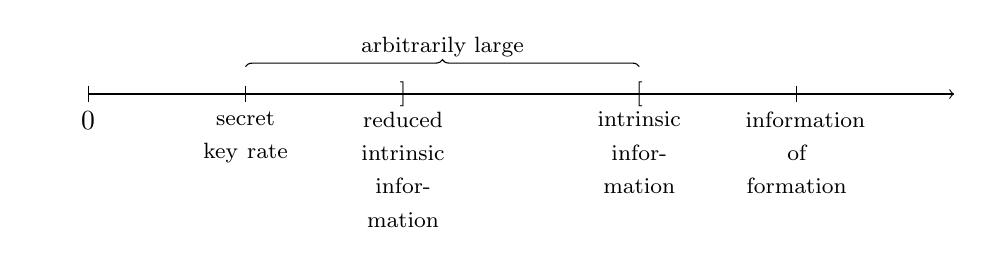
\begin{tikzpicture}

\tikzset{
    position label/.style={
       below = 3pt,
       align=center,
%       text height = 1.5ex,
%       text depth = 1ex,
       text width=13mm
    },
   brace/.style={
     decoration={brace},
     decoration={raise=3ex},
     decorate
   },
   blabel/.style={
		above = 13pt,
		align=center,
		pos=0.5   
   }
}

% draw horizontal line
\draw[->] (0,0) -- (11,0);

%draw vertical lines
\foreach \x in {0,2,9}
   \draw (\x cm,3pt) -- (\x cm,-3pt);
   
\node (foo) at (4cm,0) {\scalebox{0.9}{]}};
\node (bar) at (7cm,0) {\scalebox{0.9}{[}};

%labels
\node [position label] (Start) at (0,0) {$0$};
\node [position label] (skr) at (2,0) {\footnotesize secret key rate};
\node [position label] (rinf) at (4,0) {\footnotesize reduced intrinsic information};
\node [position label] (inf) at (7,0) {\footnotesize intrinsic information};
\node [position label] (iof) at (9,0) {\footnotesize information of formation};

\draw [brace] (skr.north) -- node [blabel] {\footnotesize arbitrarily large} (inf.north);

\end{tikzpicture}
    		\caption{The different measures for $P_{XYZ}$ and how they bound each other.}
    	\end{figure}
    	
\section{A candidate probability distribution}
    Wolf and Renner proposed in \cite{RW03} for the first time a probability distribution (Fig. \ref{Tab:candidate}) which is a good candidate for the classical analogy of \emph{bound entanglement}. 
    In fact, they offer a probability distribution that asymptotically has bound information. 
    They also show, for such a distribution, that 
    \begin{equation}
    	\keyrate{X}{Y}{Z} \neq \intrinfo{X}{Y}{Z}
    \end{equation}  
     and they emphasize that this is the first time that equality does not hold.\\
     
	\begin{figure}[h!]
	\begin{center}
		\begin{tabular}{|l r||c|c|c|c|}
		    \hline 
		    		 &	$X$ & $0$ & $1$ & $2$ & $3$ \\ 
		    $Y$ &		  &		&			&			&		\\
		    \hline 
		    \hline
		    $0$ &		   & $1/8$ & $1/8$ & $0$ & $0$ \\ 
		    \hline 
		    $1$ &		   & $1/8$ & $1/8$ & $0$ & $0$ \\ 
		    \hline 
		    $2$ &		   & $0$ & $0$ & $1/4$ & $0$ \\ 
		    \hline 
		    $3$ &		   & $0$ & $0$ & $0$ & $1/4$ \\ 
		    \hline 
		  \end{tabular} 
	\end{center}		

%\begin{table}[pos]
%\centering
%\caption{My caption}
%\label{my-label}
%\begin{tabular}{|l|l|l|l|l|l|}
%\hline
%\multicolumn{2}{|r|}{$X$} & \multirow{2}{*}{0} & \multirow{2}{*}{1} & \multirow{2}{*}{2} & \multirow{2}{*}{3} \\
%\multicolumn{2}{|l|}{Y}   &                    &                    &                    &                    \\ \hline
%\multicolumn{2}{|l|}{0}   & 1/8                & 1/8                & 0                  & 0                  \\ \hline
%\multicolumn{2}{|l|}{1}   & 1/8                & 1/8                & 0                  & 0                  \\ \hline
%\multicolumn{2}{|l|}{2}   & 0                  & 0                  & 1/4                & 0                  \\ \hline
%\multicolumn{2}{|l|}{3}   & 0                  & 0                  & 0                  & 1/4                \\ \hline
%\end{tabular}
%\end{table}
		
	    $$Z \equiv X + Y\; (mod\: 2)\; \text{ if } X,Y \in \{ 0,1\}$$ 
	    $$Z \equiv X\; (mod\: 2)\; \text{ if } X \in \{ 2,3\}$$ 
	    $$U \equiv \lfloor X/2 \rfloor $$
	    \caption{Probability distribution proposed by Renner, Wolf and Skripsky in \cite{RW03} for which it holds that $\keyrate{X}{Y}{Z} \neq \intrinfo{X}{Y}{Z}$}
	    \label{Tab:candidate}
	\end{figure}	 
	
		For this probability distribution we have
	$$ \intrinfo{X}{Y}{Z} = 3/2 ,\; \keyrate{X}{Y}{Z} = 1 , \; \redintrinfo{X}{Y}{Z} = 1 $$
	More promising is another probability they offer at the end (Fig. \ref{Tab:candidate2}) which is a slight modification of the first.
	
	
	\begin{figure}
		\begin{center}
		\begin{tabular}{|l r||c|c|c|c|}
		    \hline 
		    		 &	$X$ & $0$ & $1$ & $2$ & $3$ \\ 
		    $Y$ &		  &		&			&			&		\\
		    \hline 
		    \hline
		    $0$ &		   & $1/8$ & $1/8$ & $a$ & $a$ \\ 
		    \hline 
		    $1$ &		   & $1/8$ & $1/8$ & $a$ & $a$ \\ 
		    \hline 
		    $2$ &		   & $a$ & $a$ & $1/4$ & $0$ \\ 
		    \hline 
		    $3$ &		   & $a$ & $a$ & $0$ & $1/4$ \\ 
		    \hline 
		  \end{tabular} 
	\end{center}
	
			$$Z \equiv X + Y\; (mod\: 2)\; \text{ if } X,Y \in \{ 0,1\}$$ 
	    	$$Z \equiv X\; (mod\: 2)\; \text{ if } X,Y \in \{ 2,3\}$$ 
	    	$$Z = (X,Y) \text{ otherwise} $$
	    	
	    	\caption{A candidate probability distribution for bound information, for $a\geq 0$ (and renormalized).}
	    	\label{Tab:candidate2}
	\end{figure}
    
% done
 \chapter{A Numerical Analysis of Candidate Distributions}
 \label{ch:six}
Towards the end of the project we decided to implement a python module to do testing and analysis on some candidate probability distributions. The motivation for this was given mainly by the results showed again in \cite{RW03}. 
\section{Analysis design and goals}
    To visualize and motivate the scope of this analysis we expand Eq. \ref{eq:bounds} as follow
    \begin{equation}
    	\keyrate{X}{Y}{Z} \leq \redintrinfo{X}{Y}{Z} \leq \intrinfo{X}{Y}{Z} \leq I_{form} (X;Y|Z)
    \end{equation}
    including also the information of formation.
    As mentioned before, obtaining a value for the secret-key rate and information of formation --- the fundamental quantities for key agreement --- requires a \textit{possible} protocol. 
    For their bounds (i.e. the central parts of the inequality) we can obtain direct numerical values from the probability distribution alone. 
    The aim of this part of the project is then to take a candidate as given in Fig. \ref{Tab:candidate2} and trace the values of the reduced and normal intrinsic information for  variation of the probability distribution.\\
    
    A good result we hope to obtain is a probability distribution for which the reduced measure tends to $0$, while the intrinsic information remains larger than $0$, bounding also the information of formation to be greater than $0$. 
    Due to the tightness of the bounds, this will constrain the value for the secret key rate down to (possibly) $0$, while keeping a non-zero key cost ($I_{\text{form}}$).
    This will lead to a new candidate for bound information.\\
    
    In order to perform analysis on those measures we firstly had to implement a library of modules that dealt with the probability and information theory aspects.
    Following criteria for separability of quantum states, a quantum mechanics module was also implemented to translate and later tests the distributions from the quantum to classical regime.
    The intrinsic information (and its reduced counterpart) is defined as an \emph{infimum} over the set of tripartite probability distributions. 
    To find a correct value it would require to solve an optimization problem. 
    The definition given in section \ref{intrininfo} however does not allow us to formulate the problem as convex, or, at least, not a trivial one, since the mutual information is only convex for a fixed term.
    We decided then to adopt a Monte-Carlo method to estimate them.
     
    For each step --- i.e. for each variation --- of the candidate base probability, the values of 
    \begin{itemize}
    	\item	mutual information
    	\item	intrinsic information
    	\item	reduced intrinsic information
    	\item	trace over quantum state witness given in \cite{DPS04}
    \end{itemize}
    are estimated.
\section{Different noises analysis}

	\begin{figure}[h!]
		\centering
		\includegraphics[scale=0.5]{images/analysis-path}
		\caption{From the set $S$ of tripartite distributions we create a "path"
towards distributions with zero key cost (cyan), going through the ones without extractable key (magenta). The distributions that holds bound information reside in the cyan$\setminus$magenta part.}
		\label{Fig:analysis-path}
	\end{figure}
	The variations of the distribution mentioned above are linear steps toward a noise distribution we define.
	The first and obvious noise function we tested is the uniform distribution, which acts on all values of $P_{XYZ}$.
	Following the idea of the candidate distribution showed in Fig. \ref{Tab:candidate2} we  also utilized a noise function that operates on the non-correlated part for Alice and Bob.
	
	This method of simulating noise added to a known distribution takes also inspiration from the quantum world. 
	A method to look for bound entangled states applies a noise channel to a known entangled state and then the new state is tested on different separability criteria.
	The intuition comes from the respectively enclosed convex sets of separable states.
	
	 
	\begin{figure}
		\begin{subfigure}{0.5\textwidth}
			%Noise 1

		\begin{center}
		\begin{tabular}{|l r||c|c|c|c|}
		    \hline 
		    		 &	$X$ & $0$ & $1$ & $2$ & $3$ \\ 
		    $Y$ &		  &		&			&			&		\\
		    \hline 
		    \hline
		    $0$ &		   & $0$ & $0$ & $a$ & $a$ \\ 
		    \hline 
		    $1$ &		   & $0$ & $0$ & $a$ & $a$ \\ 
		    \hline 
		    $2$ &		   & $a$ & $a$ & $0$ & $0$ \\ 
		    \hline 
		    $3$ &		   & $a$ & $a$ & $0$ & $0$ \\ 
		    \hline 
		  \end{tabular} 
	\end{center}
			\subcaption{Noise1}
			\label{Fig:noise1}
		\end{subfigure}
		\begin{subfigure}{0.5\textwidth}
			%Noise 2

		\begin{center}
		\begin{tabular}{|l r||c|c|c|c|}
		    \hline 
		    		 &	$X$ & $0$ & $1$ & $2$ & $3$ \\ 
		    $Y$ &		  &		&			&			&		\\
		    \hline 
		    \hline
		    $0$ &		   & $a$ & $a$ & $a$ & $a$ \\ 
		    \hline 
		    $1$ &		   & $a$ & $a$ & $a$ & $a$ \\ 
		    \hline 
		    $2$ &		   & $a$ & $a$ & $0$ & $0$ \\ 
		    \hline 
		    $3$ &		   & $a$ & $a$ & $0$ & $0$ \\ 
		    \hline 
		  \end{tabular} 
	\end{center}
			\subcaption{Noise2}
			\label{Fig:noise2}
		\end{subfigure}
		\caption{Different noises disturbs different parts of the correlation between $X$ and $Y$}
		\label{Fig:noises}
	\end{figure}
	
\section{The problem with the reduced intrinsic information}
    During the implementation of the module we were confronted with some issues on the measure of the reduced intrinsic information.
    Recalling Eq. \ref{eq:reducedintrinfo}, we first generate random channels $XYZ \rightarrow U$ to get the conditional probability $P_{U|XYZ}$. 
%    In some cases, also a channel $X\rightarrow U$, or $XY \rightarrow U$ can be used.
    Then the intrinsic information is minimized over all possible channels $ZU \rightarrow \bar{ZU}$.
    Ideally, we want to show how the reduced intrinsic information goes to $0$, so that the secret key rate also falls to $0$. 
    Thus, $\Ent (U)$ is a lower bound on the value of the reduced intrinsic information.
    Since $U$ is generated through an arbitrary channel, however, it will not have $\Ent (U) = 0$.
    In order to minimize this lower bound, the marginal $P_U$ should be deterministic.
    
    Observing this, we questioned the usefulness of the reduced intrinsic information as a measure to demonstrate the existence of bound information, contrary to we thought at the beginning. 
    
\section{Results}
Despite the difficulties encountered in implementing the code, we were able to produce some marginal results.
When the noise functions were applied to the marginal $P_{XYZ}$ of the distribution in Fig. \ref{Tab:candidate} we were able to make the following observations
\begin{itemize}
\item For the uniform noise, as expected, the behaviour presents no intrinsic information nor reduced intrinsic information. The two measures remain the same until around $\alpha = 1- 1/8 = 0.875$. Around that point the reduced intrinsic information of the behaviour \textit{decrases} until reaching $1$, as we already knew from \cite{RW03}.

\item For the noise in Fig. \ref{Fig:noise1}, we notice first of all that the intrinsic information is not monotonic along the path. It takes the form of a convex function with minimum for an $\alpha$ around $0.4$. At both ends of the path the two measures diverge resulting in $\intrinfo{X}{Y}{Z} \approx 1$ and $\redintrinfo{X}{Y}{Z} \approx 0.5$ for $\alpha = 0$, i.e. for just the noise function represented in the figure. On the other end we obtain again the results as before for the marginal of the candidate.

\item Finally for the noise function in fig. \ref{Fig:noise2} ... %TODO to measure
\end{itemize}

%TODO put images
    
    
% empty
% \chapter{Conclusion}
% Throughout the project, topics of information theory and quantum mechanics were researched thoroughly.
We have built an understanding why some aspects of quantum mechanics present an analog in classical key agreement and how they can be used as an intuition in research.
Moreover, we have seen how and why the question of bound information remains yet an open question.
We researched and understood the measures presented as bounds to define the amount of secrecy a probability distribution among parties can hold, and how much does it cost to build it.
Lastly, the implementation of a python library to perform a  numerical analysis of candidates was instrumental to observe how the measure of reduced intrinsic information is not a useful measure for the search of bound information.\\

As future work on the topic, more thought can be put into the usefulness of the reduced intrinsic information measure.
The intuitions on the bounds on $\Ent(U)$ and the minimization of the term $\intrinfo{X}{Y}{ZU}$ have to be formally stated.
The code produced during the project, while providing as a library of functions for the study, was not completed to the intended form, as it only tested the marginal of \ref{Tab:candidate} and not the tripartite distribution \ref{Tab:candidate2}.
More development can be done in the library to be able to test other candidate tripartite distributions.
More tests for separability criteria of the translated quantum states are already being added as a continuation of the work.

\begin{appendices}
	\chapter{Mathematical Framework for QM}
	
\section{Mathematical Framework (for QM)}
	
%	\begin{enumerate}
%	\item Dirac's braket notation
%	\item Inner/(Outer) product
%	\item Linear operator
%	\item Adjoints and Hermitian operators
%	\item Pauli matrices
%	\item Tensor Product and tensor space
%	\end{enumerate}
	
	
	\section{Inner product spaces}
	In standard vector notation we define the inner (scalar) product of complex vectors as
	$$ ( \vec{v}, \vec{w} ) =  \begin{pmatrix} \bar{v_1} & \bar{v_2}\end{pmatrix} \begin{pmatrix} w_1 \\ w_2 \end{pmatrix} = \begin{pmatrix} \bar{w_1} & \bar{w_2}\end{pmatrix} \begin{pmatrix} v_1 \\ v_2 \end{pmatrix} = ( \vec{w}, \vec{v} )^{\dagger}$$
	Where $\dagger$ represents the conjugate transpose.\\
%	This property is fundamental in the sense that it will allows us to go from a state space --- that can be many dimensional --- to a \textit{measurement} space, which assumes real values.\\ %0 and 1 in our case??
	
	It is important also to note that through the inner product of two vectors we also define the norm $\|\ket{v}\|  =  \sqrt{( \vec{v}, \vec{v} )} $.\\
	
	
	The outer product of two vectors, on the other hand, produces a matrix, with very important properties.  
	
	\section{Tensor product spaces}
	The tensor product $V\otimes W$ is an operation between vector spaces that combines every element of the first vector space and every element of the second vector space in a bigger vector space. Tensor product is linear and from its properties emerges the famous phenomenon of quantum entanglement, which simply is that not all vectors in $\H = V\otimes W$ can be divided into $\ket{v}\otimes\ket{w}$ with $\ket{v}\in V,\; \ket{w}\in W$. This will later be explained in the next section.\\
	Notation and abbreviation for the tensor product is 
	$$ \ket{v}\otimes\ket{w} = \ket{v}\ket{w} = \ket{v,w} = \ket{vw}$$
	It has the following properties:
	\begin{description}
		\item $\forall\ket{v}\in V ,\; \forall\ket{w}\in W, \; \forall z\in \mathbb{C}$	\\
					$ z(\ket{v}\otimes\ket{w}) = (z\ket{v})\otimes\ket{w} = \ket{v}\otimes(z\ket{w} $
		\item $\forall\ket{v_1},\ket{v_2}\in V ,\; \forall\ket{w}\in W$	\\
					$ (\ket{v_1} + \ket{v_2})\otimes\ket{w} = \ket{v_1w} + \ket{v_2w} $
		\item $\forall\ket{v}\in V ,\; \forall\ket{w}\in W, \; A:V\rightarrow V' \; B:W\rightarrow W'$	\\
					$ (A\otimes B) \left(\sum_i a_i \ket{v_i w_i} \right) = \sum_i a_i A\ket{v_i}\otimes B\ket{w_i} $
	\end{description}
	The inner product on $V$ and $W$ can be used to define (linearly) an inner product on $V\otimes W$.	
	
\section{Quantum Mechanics}
	%TODO Correct and reformulate this
	
	
	
	%TODO review this
	All pure states in QM are normalized vectors in $\H$.
	$$ \ket{\psi} \text{ is a state vector } \Rightarrow \ket{\psi}\in\H \text{ and }  \vert\bk{\psi}{\psi}\vert = 1$$
	This is instrumental in seeing them as probability vectors. Every linear operator has then to be unitary to maintain this property.\\
	A statistical mixture of states corresponds to a \emph{density matrix}, which is itself a new state. It is important to note that a mixture of probability of states is not the same thing as superposition of states. In the latter we don't have a measure of uncertainty of the state, meaning also that in theory we are always able to find a measurement basis that will always output the same result for that state. In the former, however, this is not possible given by the direct intrinsic uncertainty of the state.\\
	Density matrices have then the properties:
	$$ M = \rho = \sum_i p_i \ketbra{\psi_i}{\psi_i} = \sum_i p_i P_{\ket{\psi_i}} \text{  , where state }\ket{\psi_i}\text{ has probability } p_i $$ 
	$\rho$ is a positive, trace-1 operator meaning that $\Tr{\rho} = 1$ and all eigenvalues of $\rho$ are positive. Moreover $\rho$ is a linear combination of projectors $\proj{\psi_i}$ which makes $\rho\in\mathbf{P}(\H)$ a projector itself on the the Hilbert space.
	
		\subsection{Quantum Measurements}
		To get an actual value out of a qubit one has to \textit{measure} it. Measurement is, mathematically, a projection onto some chosen computational basis. The result for each base vector projection is then interpreted as a \emph{probability}. The state then changes after measurement, meaning for example that it will not retain it value as superposition any more.\\
		...\\
		
		If Alice has the state $\ket{psi_i}$ out of $i=1..n$ and all states are orthonormal, then Bob can find out what the choice of $i$ was.
		If the states are not orthonormal there is no quantum measurement capable of distinguishing the states. \\
		From this follows that if the states $\ket{\psi_1}$ and $\ket{\psi_2}$ are not orthogonal, then $\ket{\psi_2}$ has a component orthogonal to $\ket{\psi_1}$ but also a component parallel to it which will give probability not $0$ of measuring differently.
		
			\begin{xmpl}
      \begin{equation*} % environment for equation 
				Z = \begin{bmatrix} 1 & 0 \\ 0 & -1 \end{bmatrix} \quad P_{+1} = \proj{0} , \; P_{-1} = \proj{1}
      \end{equation*}
				Measurement on qubit $ \ket{\psi} = \frac{\ket0 + \ket1}{\sqrt{2}} $ has probability $p_{+1} = \bra{\psi}P_{+1}\ket{\psi} = \bk{\psi}{0}\bk{0}{\psi} = \frac{1}{2}$ and similarly $p_{-1} = \frac{1}{2}$
				\cite{NC10}
			\end{xmpl}
	


	\chapter{Quantum Mechanics}
	\section{Dirac's notation}
    \lipsum[8]
\section{Measurements on a  basis}
    \lipsum[7]
\section{Quantum entanglement}
    \lipsum{4}

%	\chapter{Information Theory}
%	\input{chapters/appendixC}
\end{appendices}

%\bibliographystyle{apalike}
\printbibliography
\end{document}
